% Chapter 3

\chapter{SCATS Volume Data} % Main chapter title

% For referencing the chapter elsewhere, use \ref{Chapter3}
\label{Chapter3}

% This is for the header on each page - perhaps a shortened title
\lhead{Chapter 3. \emph{SCATS Volume Data}}

%----------------------------------------------------------------------------------------
% Quotation
``There is no order in the world around us, we must adapt ourselves to the requirements of chaos
instead."

\begin{flushright}
Kurt Vonnegut, \textit{Breakfast of Champions} (1973)
\end{flushright}

%---------------------------------------------------------------------------------------------------
%	CONTENT
%   Reference - http://www.scats.com.au/files/an_introduction_to_scats_6.pdf
%---------------------------------------------------------------------------------------------------
\section{Introduction}
SCATS(Sydney Coordinated Adaptive Traffic System) is an adaptive traffic control system. It was
developed by the Department of Main Roads in the 1970's. SCATS operates in real-time by adjusting
signal timings in response to changes in traffic demand and road capacity. All major and minor
cities in Australia and New Zealand use SCATS. Few other cities around the world such as Hong
Kong, Kuala Lumpur, Sanghai and Singapore also have adopted SCATS over other adaptive traffic
control system. In Melbourne and surrounding cities, SCATS controls more than 3,900 sets of traffic
signals

There are three main parameters that SCATS user to achieve traffic signal coordination:
\begin{itemize}
\item[\tiny{$\blacksquare$}] Cycle time: The total time of all signal sequences in a cycle
\item[\tiny{$\blacksquare$}] Phase split: The proportion of the cycle time allocated to each phase
\item[\tiny{$\blacksquare$}] Offset: The time relationship between the starting and finishing of
the green phases of succesive sets of signals within a coordinated system
\end{itemize}

The desicion making of the SCATS system occurs at two levels - \emph{strategic} and \emph{tactical}.


\section{Volume data}
Traffic loop detectors are embedded in the raod pavement and located in each lane near the stop
line at traffic intersections. These detectors collect traffic volume and the time it takes a
vehicle to clear the loop. In this research we used the data collected from sensors at 1084
homogeneous links(a road segment where the volume for all traffic along that link is collected).
Traffic volume was collected for every 15 minutes interval from 01/01/2008 to 25/07/2013, a total
of 195168 observations.


\subsection{Handling missing data}


\section{Exploratory analysis}
In this section, we will perform soem

Figure \ref{fig:AverageTrafficVolume} shows the daily, weekly, monthly and yearly average traffic
volume at a site location.Figure \ref{fig:TypicalDayTraffic} shows how a typical day of the week
on average looks like at a homogeneous link. We will explore both the south and north bound
traffic data at Nicholson street (north of Melbourne's CBD)between Gertrude street and
Victoria Parade  during the period 01/01/2008 to 25/07/2013.

\begin{figure}[h]
    \centering
    \subfloat[Daily][Daily]{
    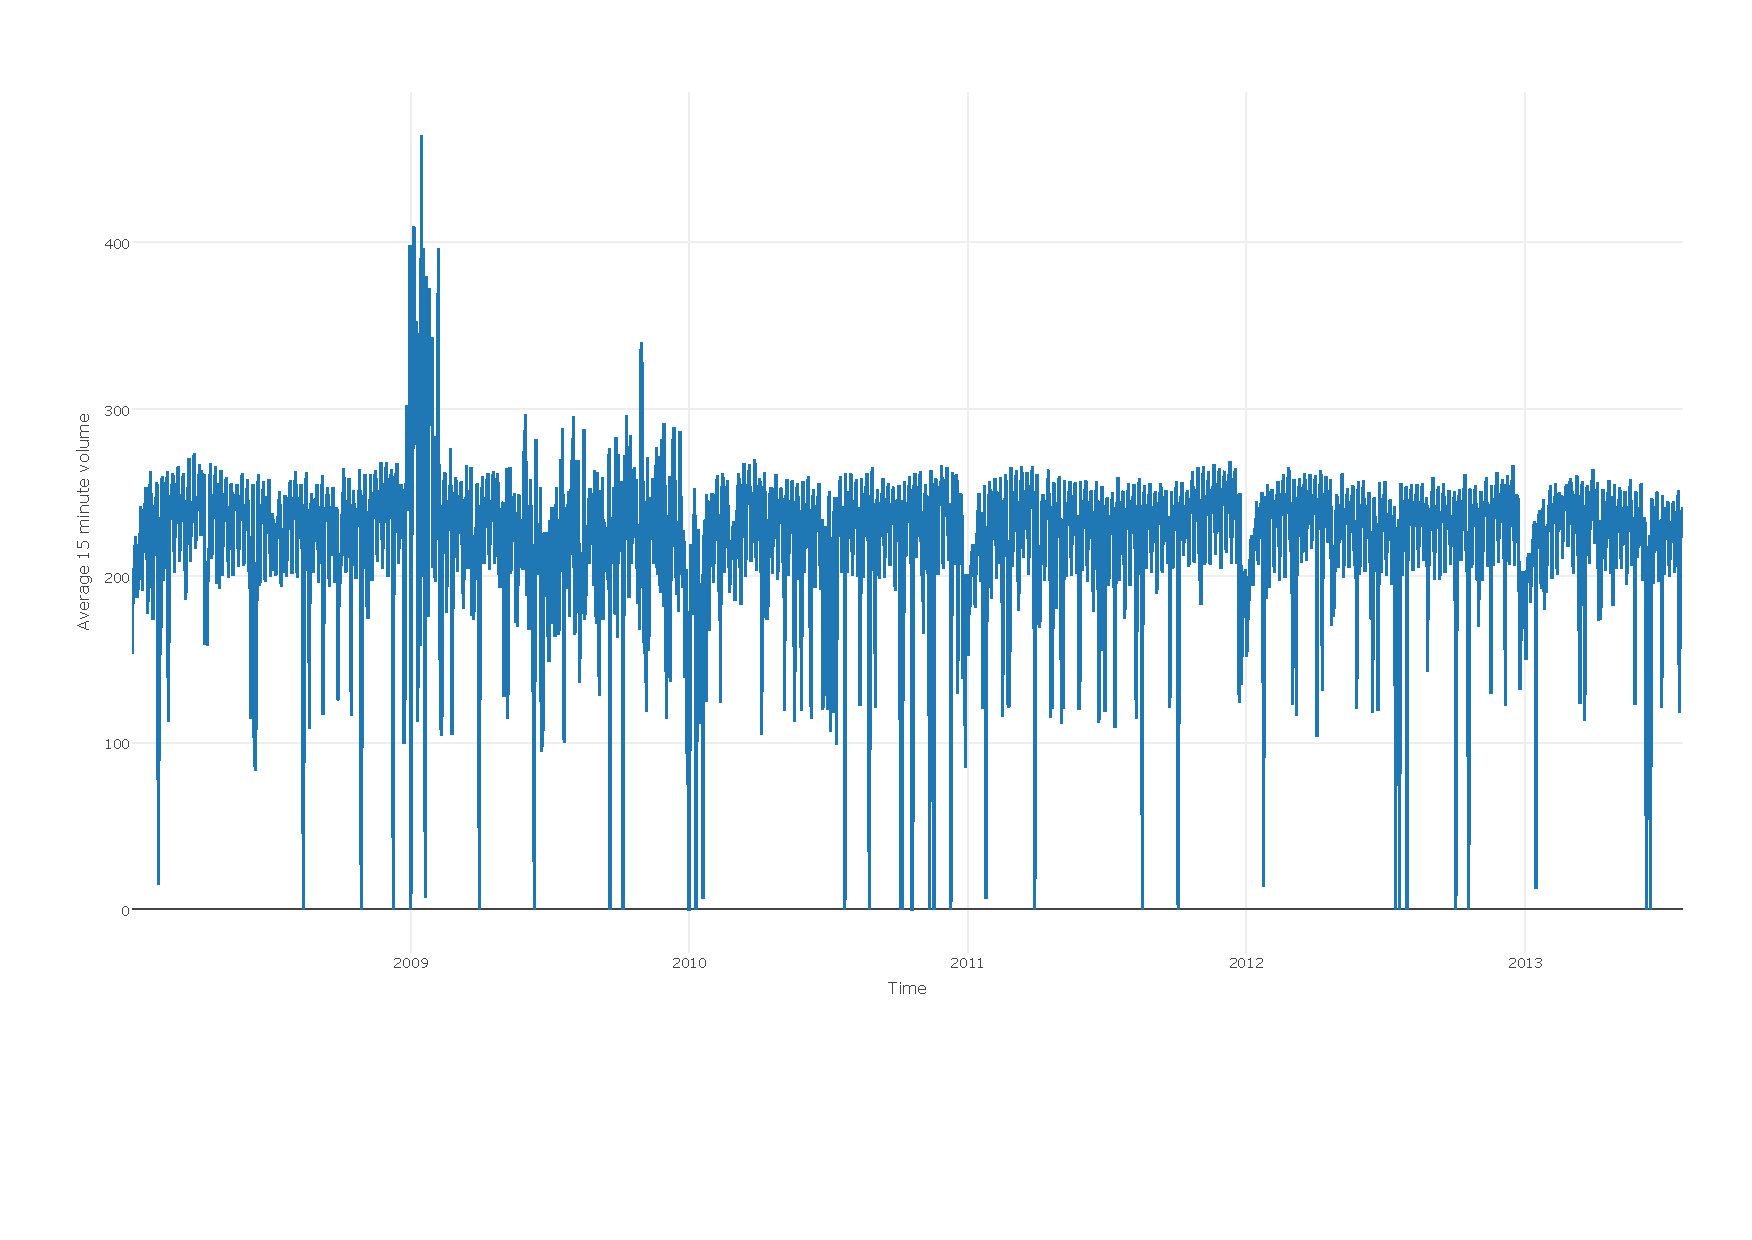
\includegraphics[width=0.4\textwidth]{Figures/averages-daily.pdf}
    \label{fig:AverageDaily}}
    \qquad
    \subfloat[Weekly][Weekly]{
    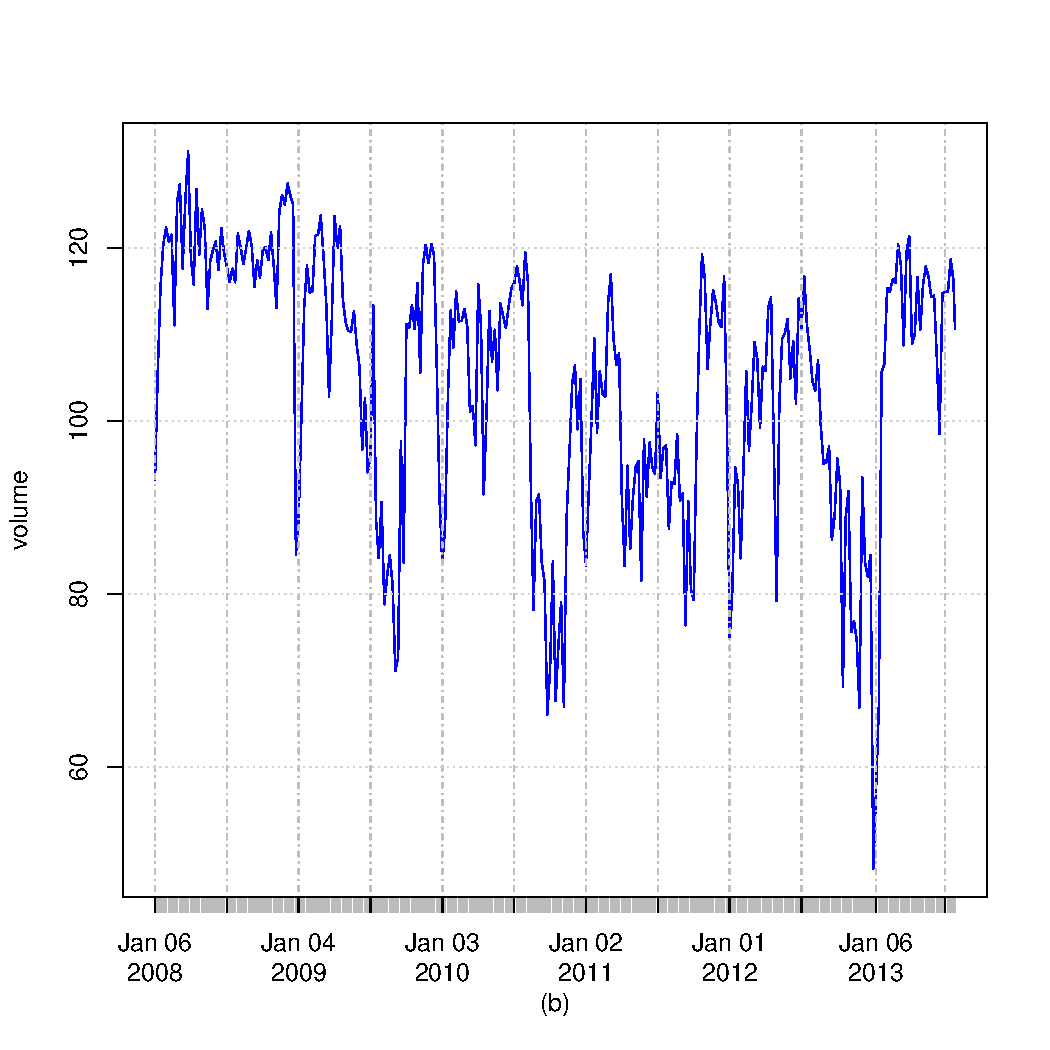
\includegraphics[width=0.4\textwidth]{Figures/averages-weekly.pdf}
    \label{fig:AverageWeekly}}

    \subfloat[Monthly][Monthly]{
    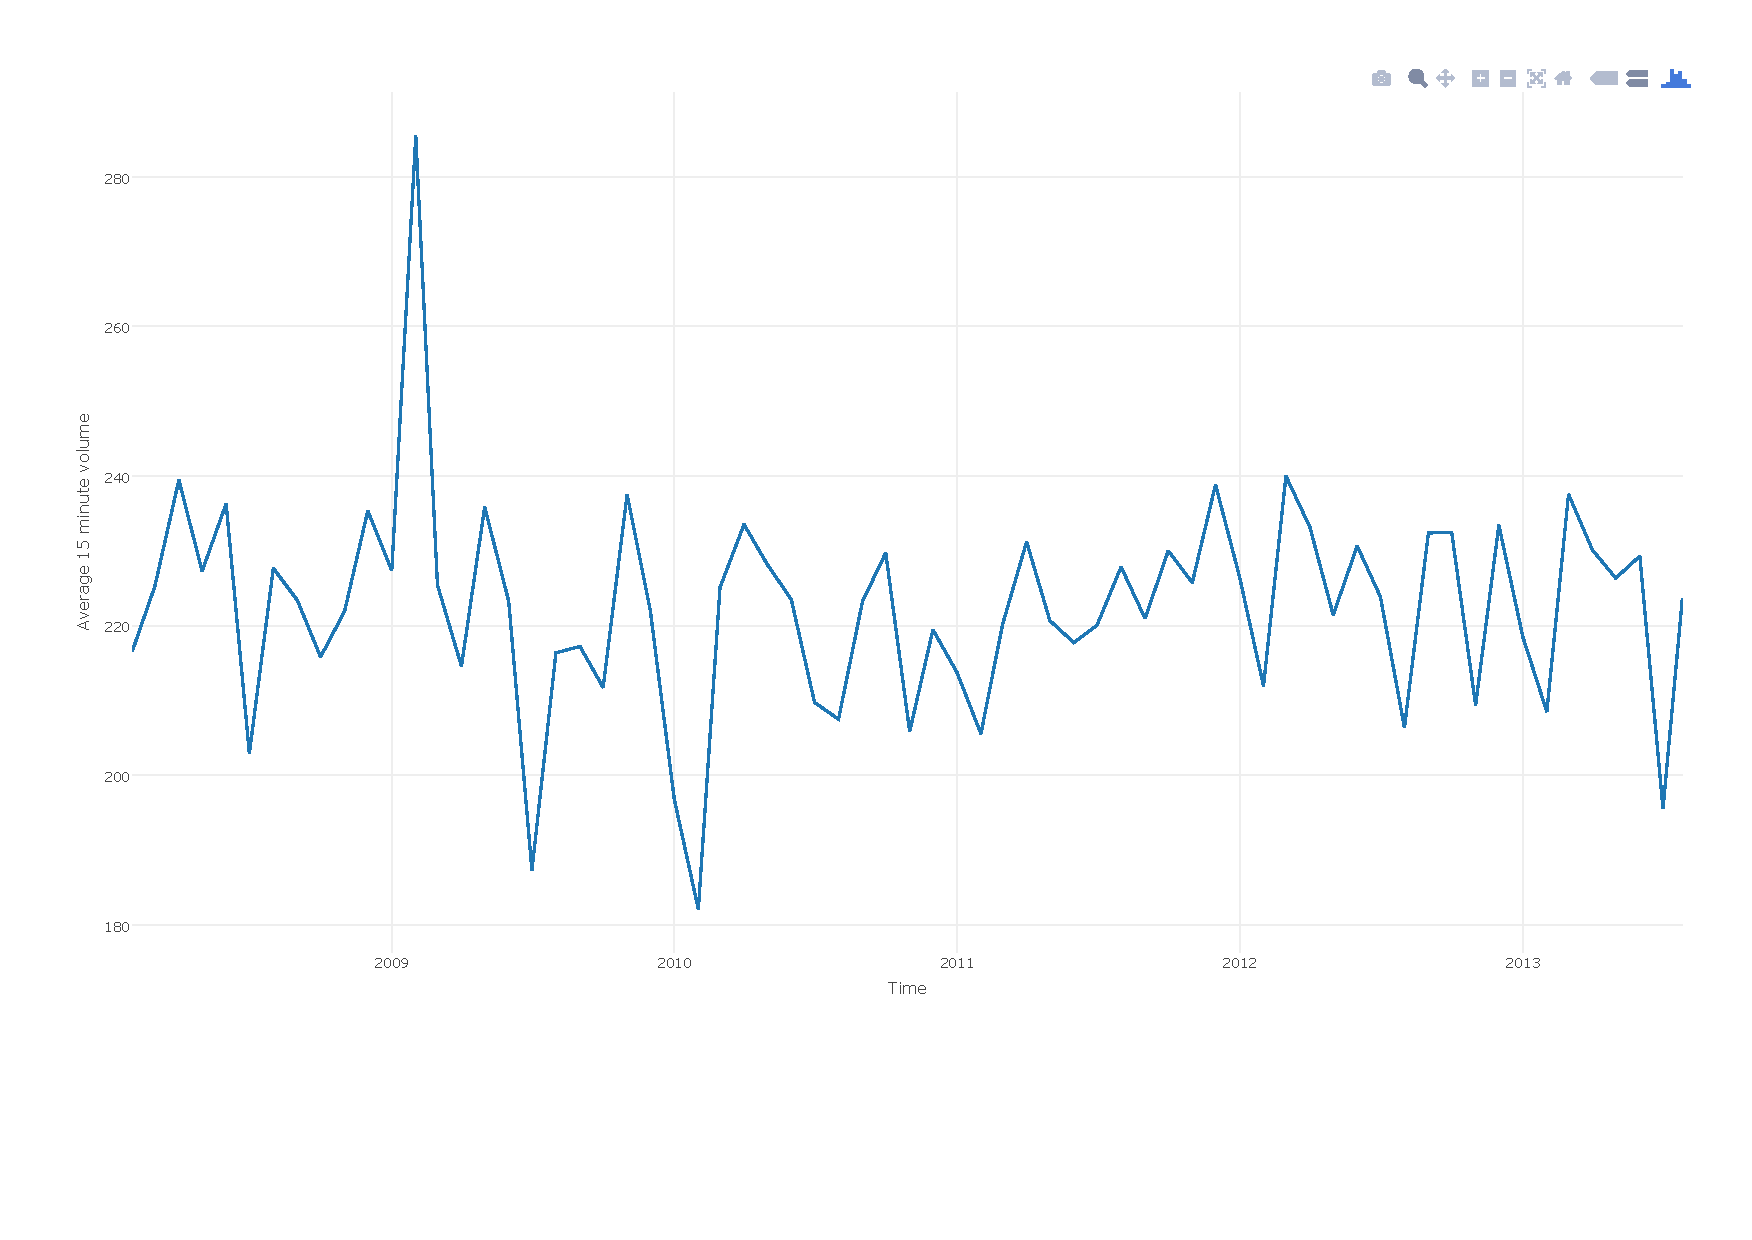
\includegraphics[width=0.4\textwidth]{Figures/averages-monthly.pdf}
    \label{fig:AverageMonthly}}
    \qquad
    \subfloat[Yearly][Yearly]{
    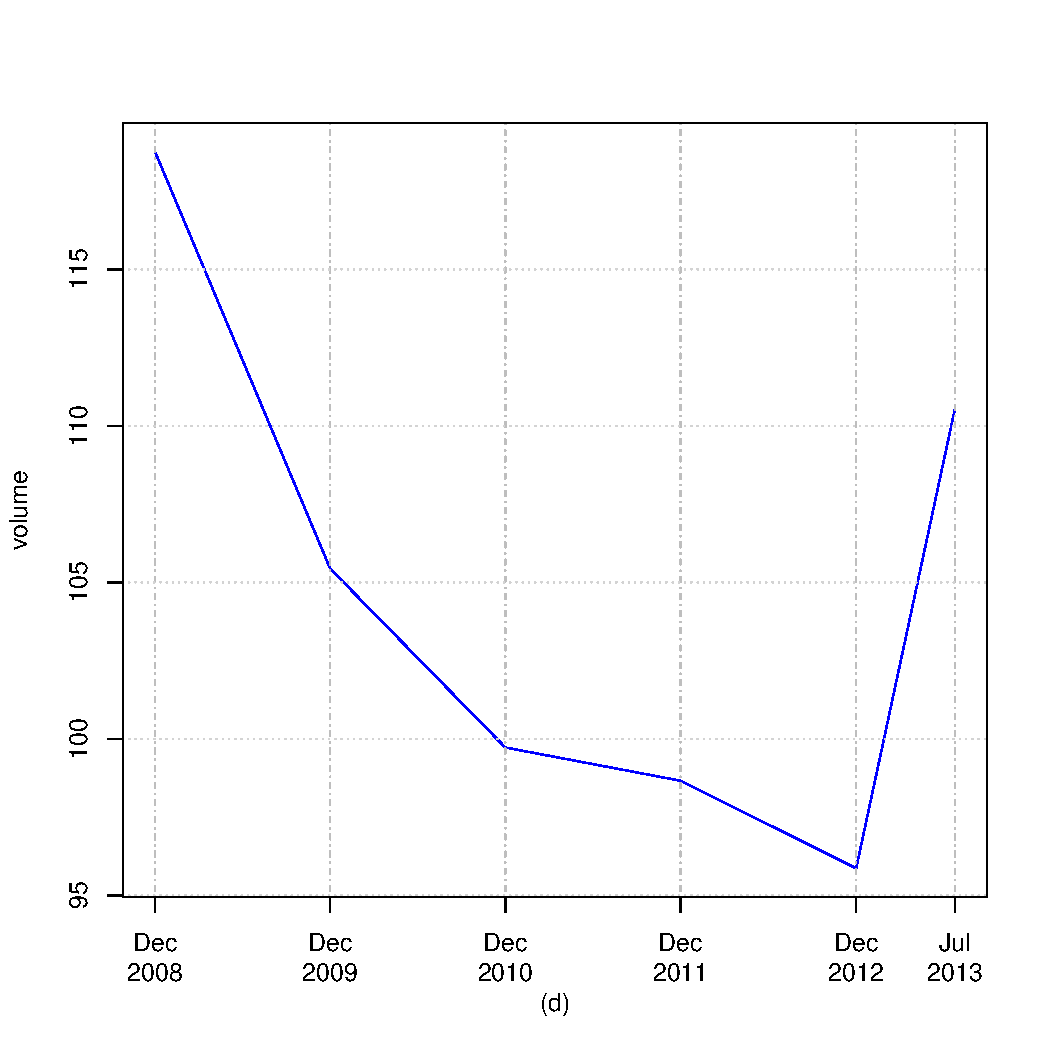
\includegraphics[width=0.4\textwidth]{Figures/averages-yearly.pdf}
    \label{fig:AverageYearly}}

    \caption[Average Traffic Volume]{(a) daily, (b) weekly, (c) monthly and (d) yearly average of
    traffic volume (15 mins interval) at a site location from the period 01/01/2008 to 26/07/2013}
   \label{fig:AverageTrafficVolume}
\end{figure}

\begin{figure}[h]
    \centering
    \subfloat[Monday][Monday]{
    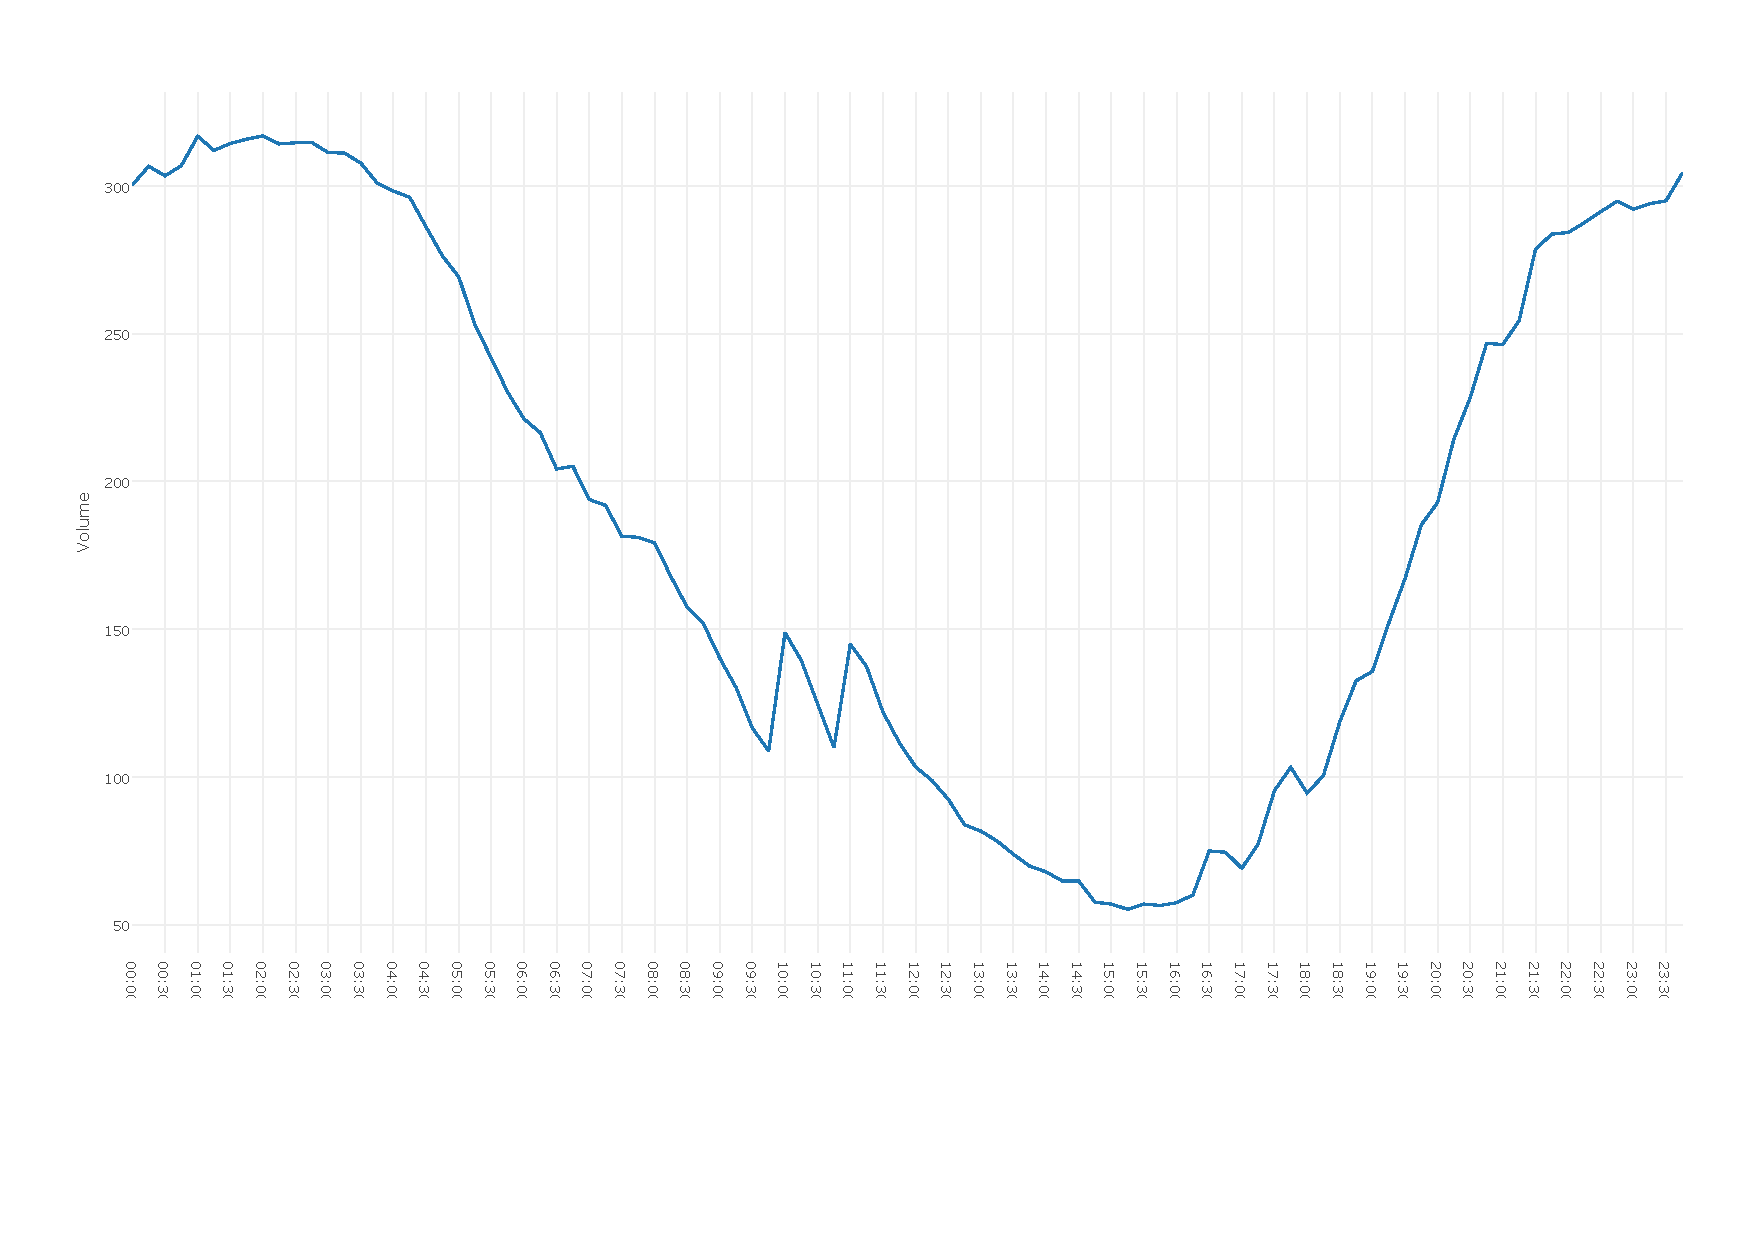
\includegraphics[width=0.4\textwidth]{Figures/typical-Monday.pdf}
    \label{fig:typicalMonday}}
    \qquad
    \subfloat[Tuesday][Tuesday]{
    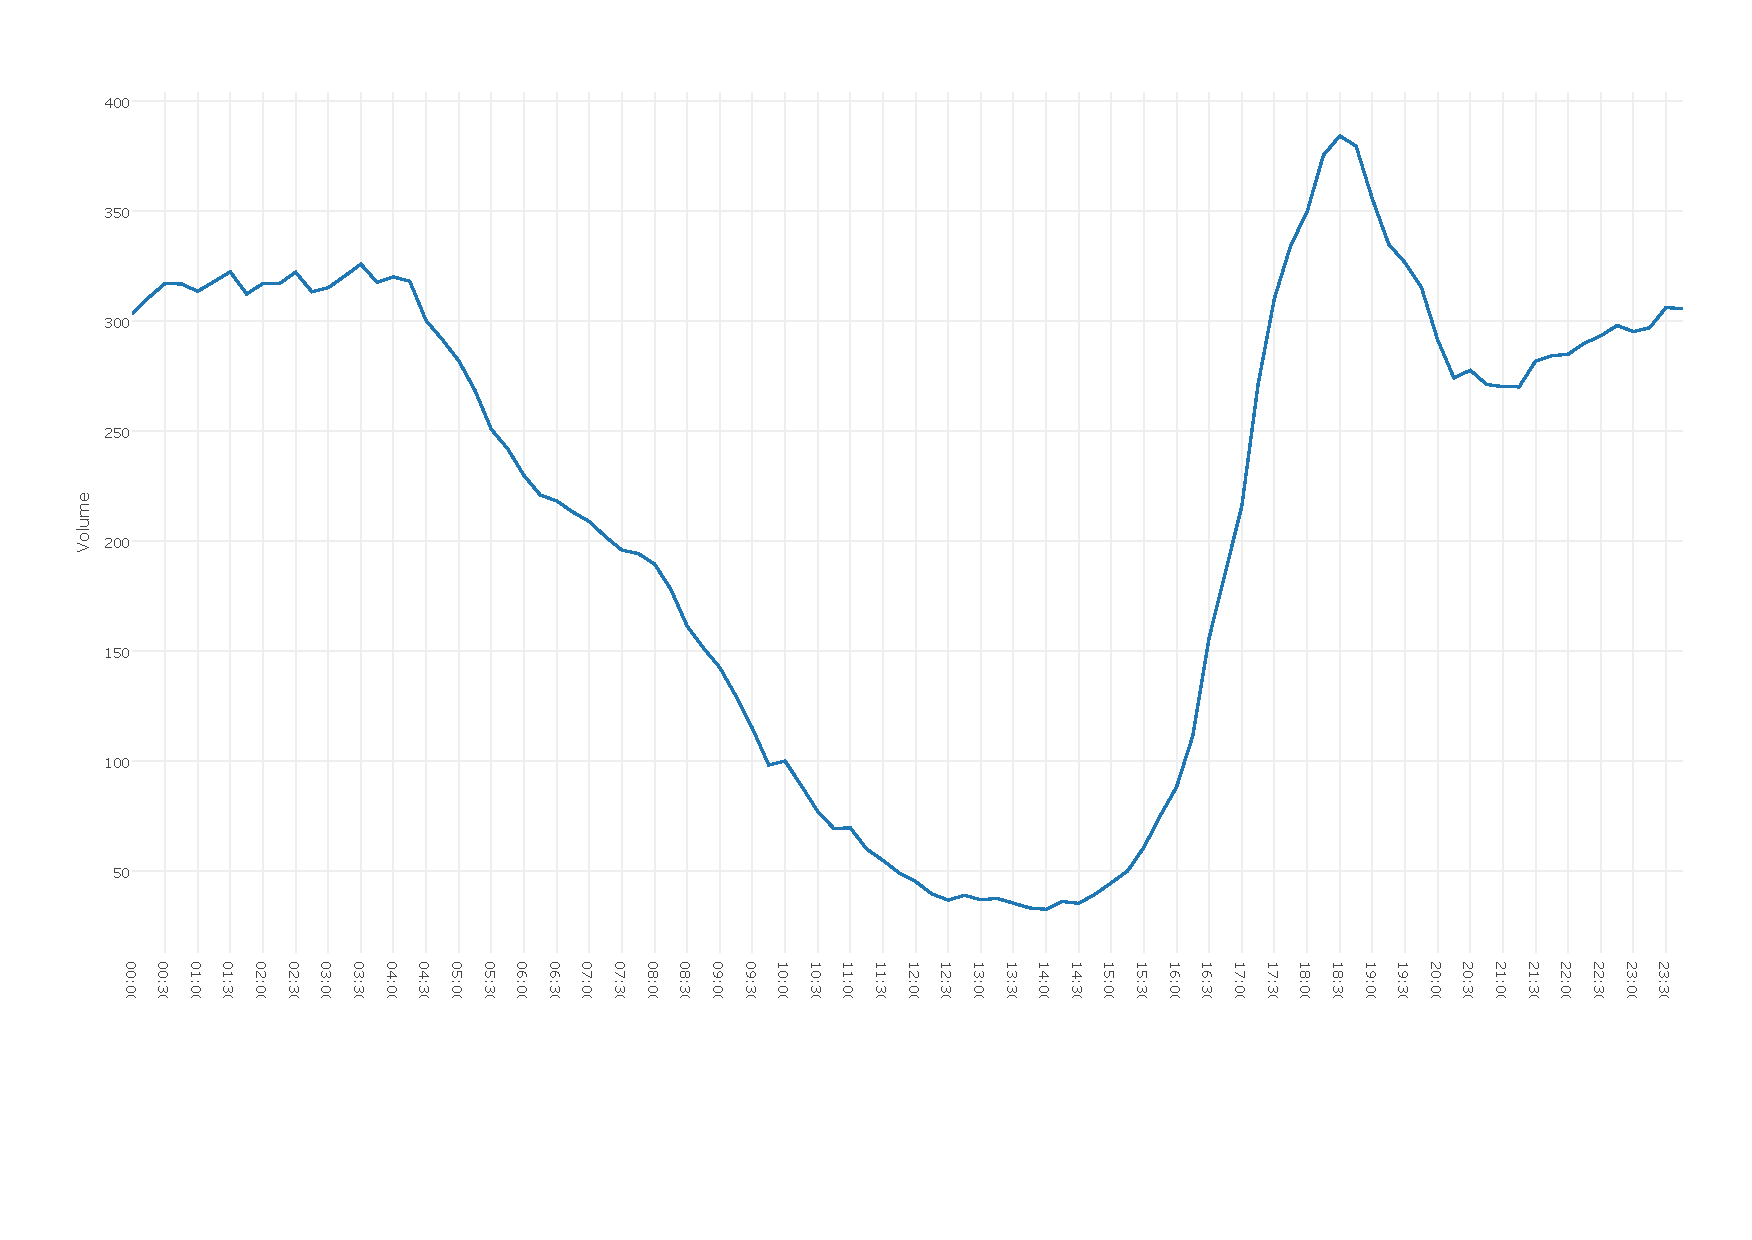
\includegraphics[width=0.4\textwidth]{Figures/typical-Tuesday.pdf}
    \label{fig:typicalTuesday}}

    \subfloat[Wednesday][Wednesday]{
    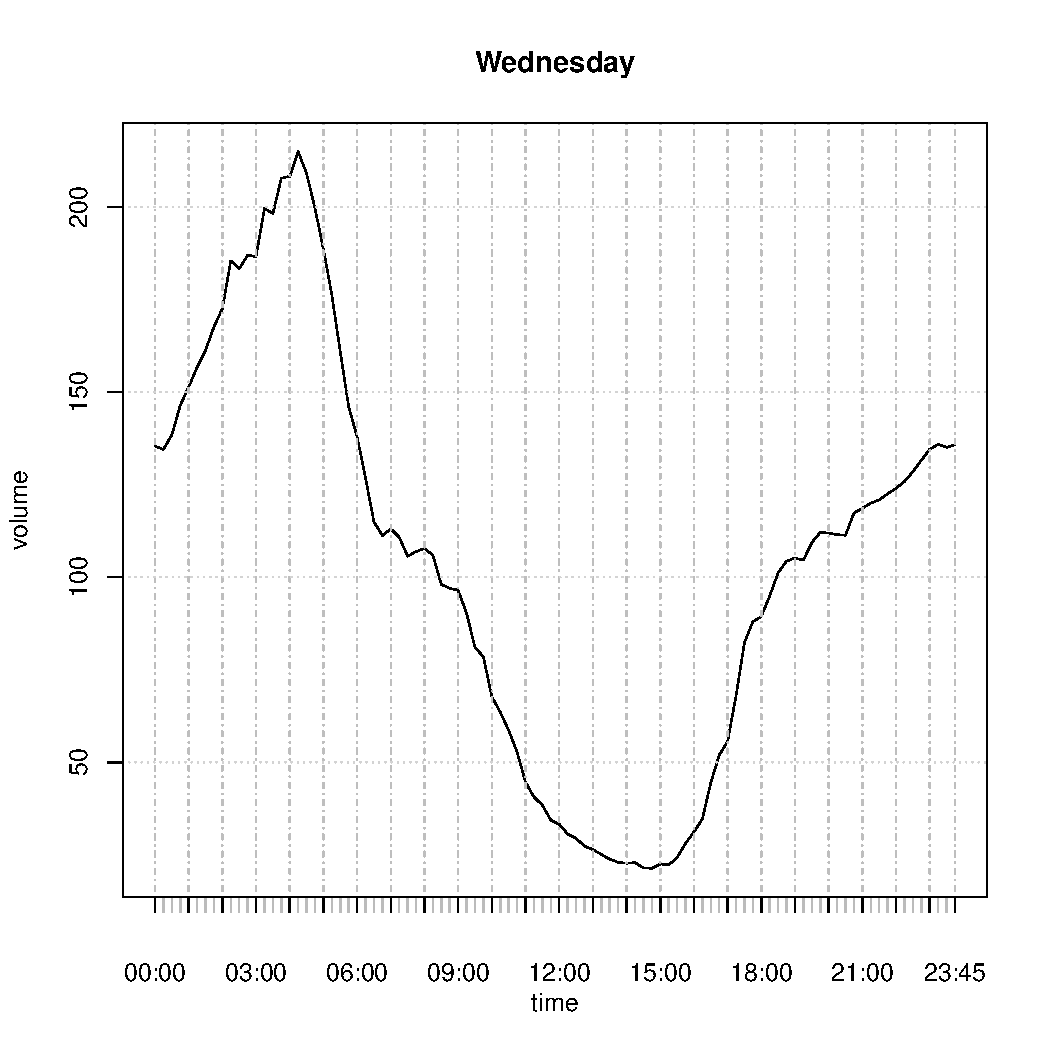
\includegraphics[width=0.4\textwidth]{Figures/typical-Wednesday.pdf}
    \label{fig:typicalWednesday}}
    \qquad
    \subfloat[Thursday][Thursday]{
    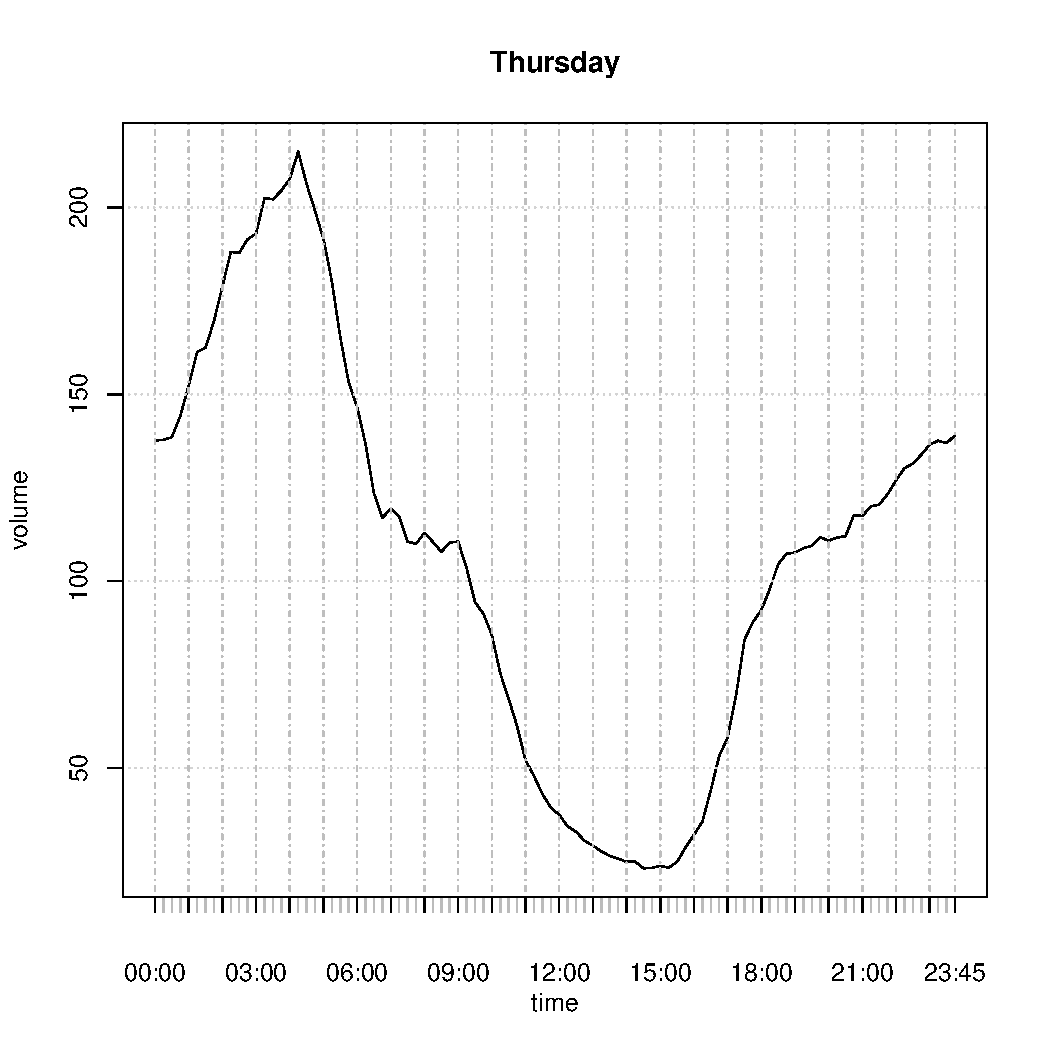
\includegraphics[width=0.4\textwidth]{Figures/typical-Thursday.pdf}
    \label{fig:typicalThursday}}

    \subfloat[Friday][Friday]{
    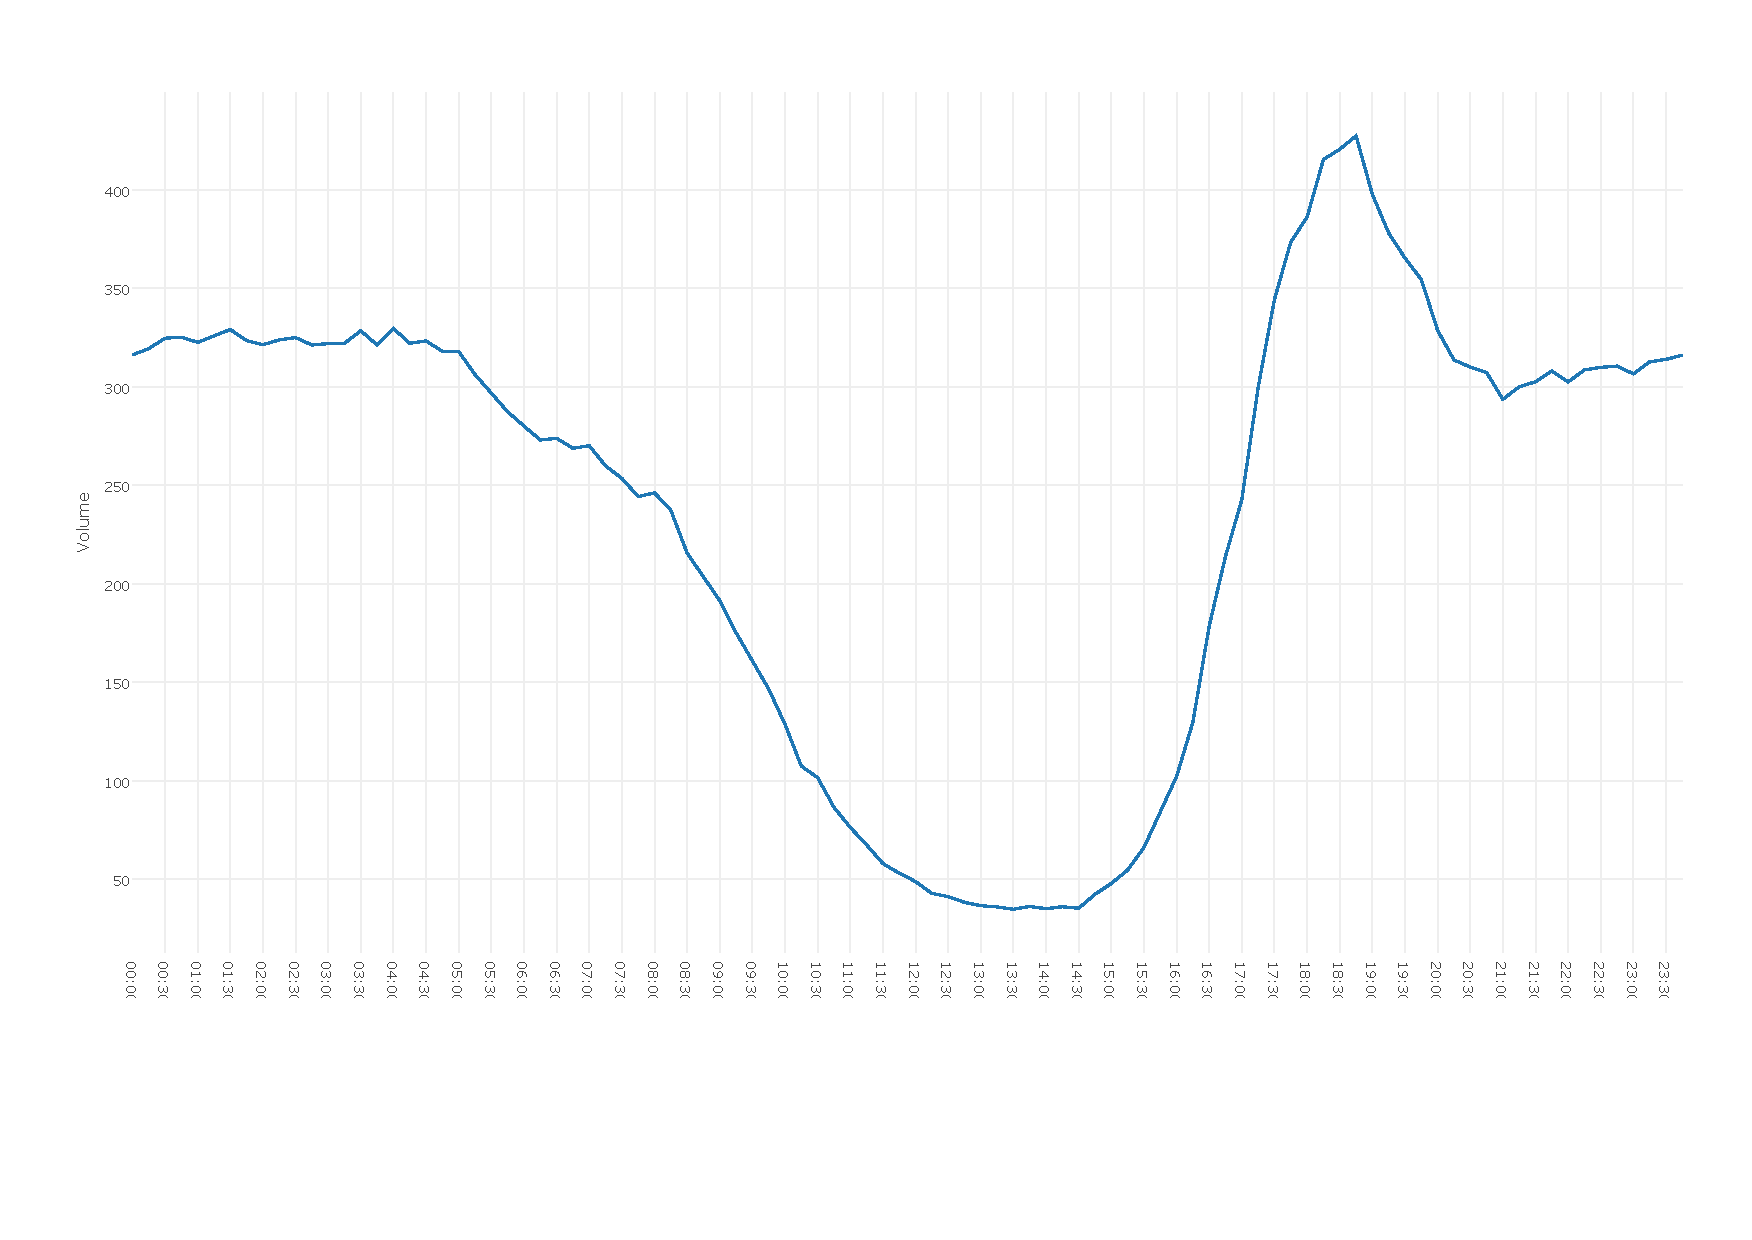
\includegraphics[width=0.4\textwidth]{Figures/typical-Friday.pdf}
    \label{fig:typicalFriday}}
    \qquad
    \subfloat[Saturday][Saturday]{
    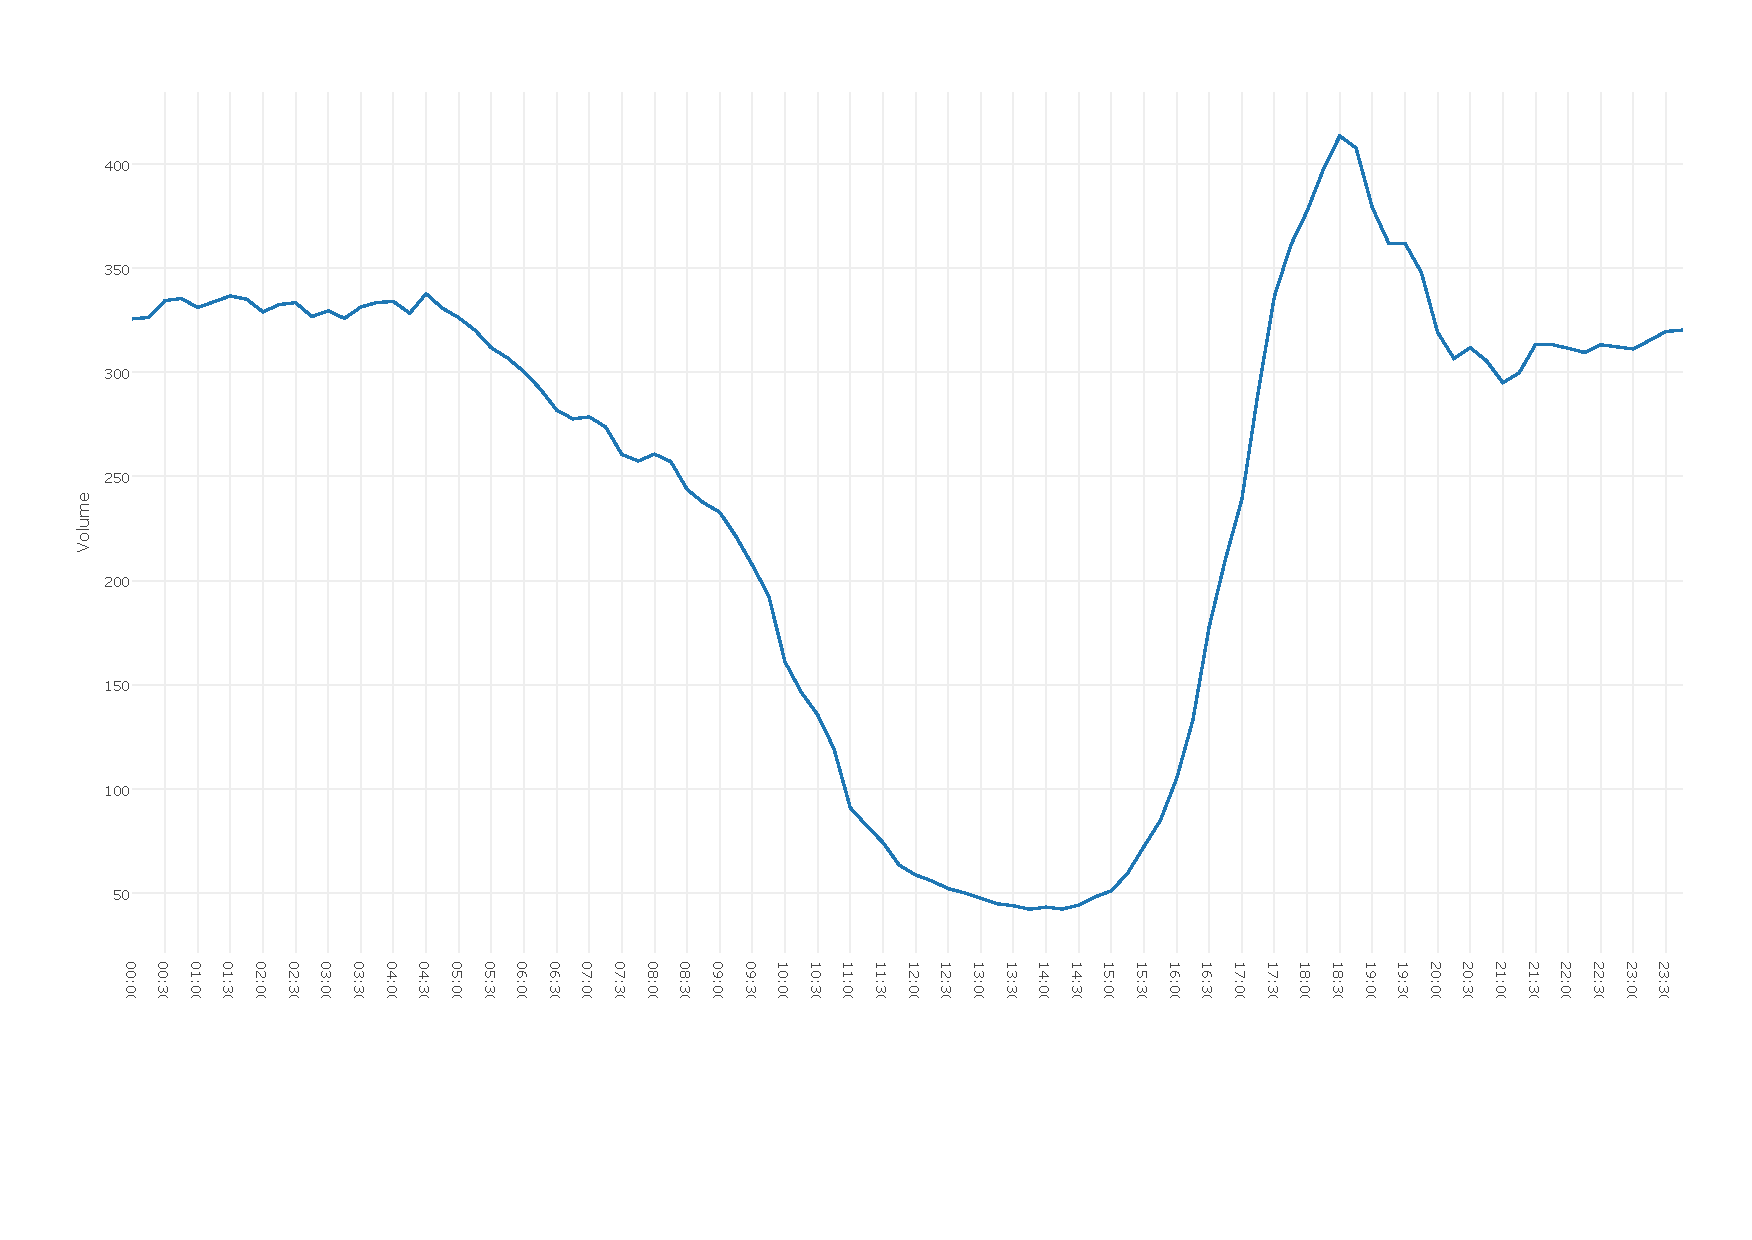
\includegraphics[width=0.4\textwidth]{Figures/typical-Saturday.pdf}
    \label{fig:typicalSaturday}}

    \caption[Average traffic grouped by every day of the week]{Average traffic grouped by every
    day of the week.}
    \label{fig:TypicalDayTraffic}
\end{figure}

\begin{figure}[h]
    \centering
    \subfloat[ACF][ACF]{
    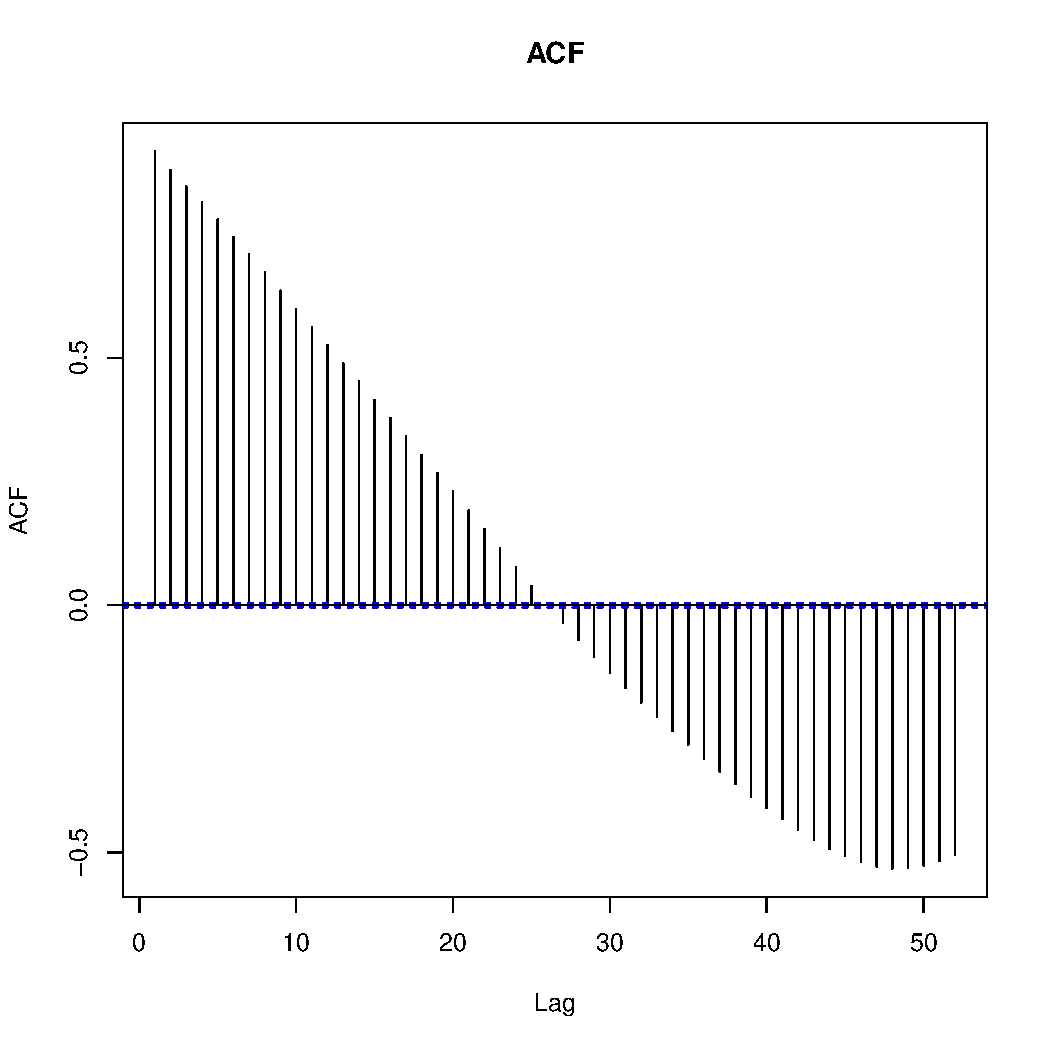
\includegraphics[width=0.4\textwidth]{Figures/acf.pdf}
    \label{fig:acf}}
    \qquad
    \subfloat[PACF][PACF]{
    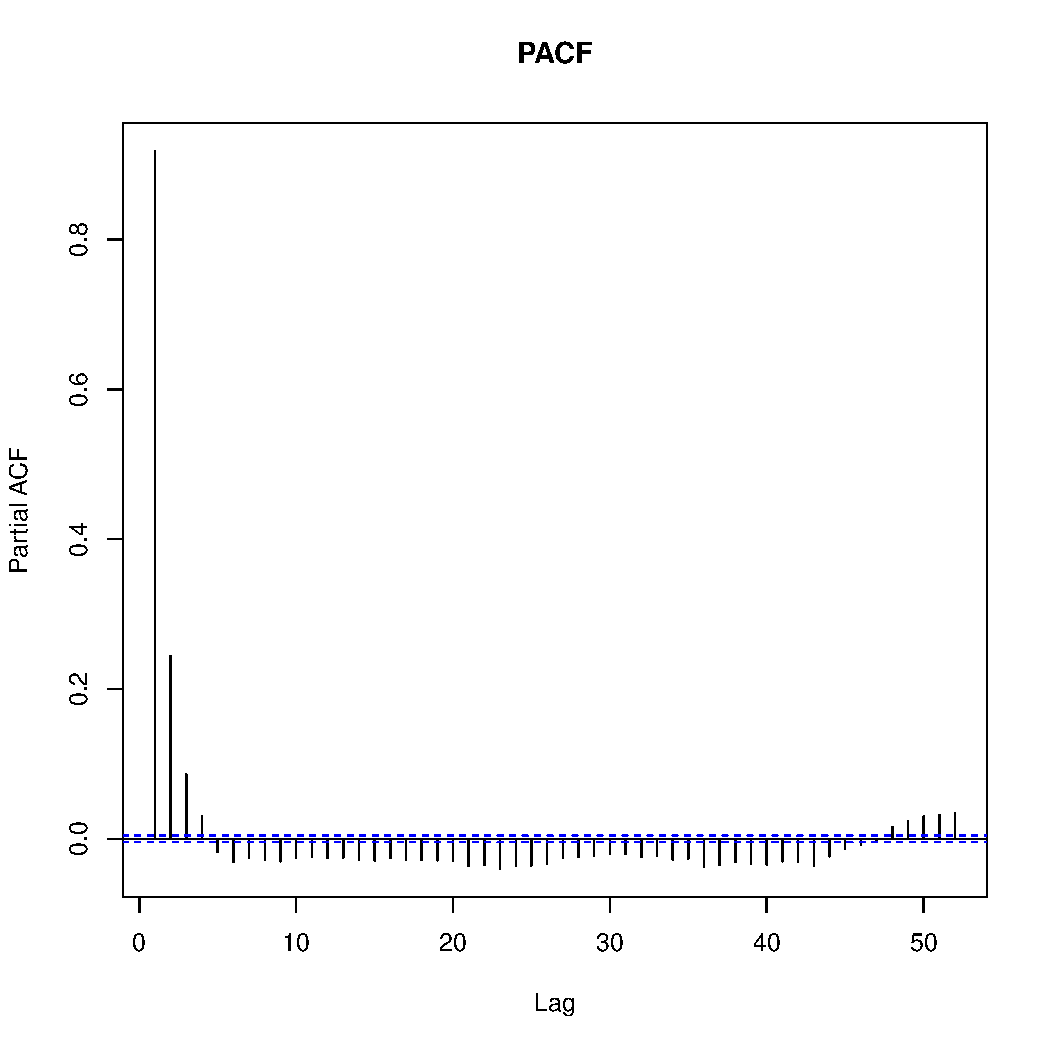
\includegraphics[width=0.4\textwidth]{Figures/pacf.pdf}
    \label{fig:pacf}}

   \caption[Plots of ACF and PACF]{Plots of the autocorrelation and partial autocorrelation
   functions}
   \label{fig:acfPacf}
\end{figure}